\begin{columns}[t]
	\begin{column}{0.5\textwidth}
		\begin{block}{\large Motivation}
		    \begin{columns}[t]
			    \begin{column}{0.62\textwidth}
			    	\vspace{-0.2in}
					    \begin{itemize}
							\item \textbf{Objective}: Improve the per iteration performance of a kinodynamic planner.
					    	\item \textbf{Key idea}: Instead of random propagation, compute local maneuvers that balance an exploitation-exploration trade-off
					    	\item Exploitation maneuvers guide the system towards the goal given local heuristic information
					    	\item Exploration maneuvers move the system in different directions to deal with situations where heuristic does not provide good guidance.
					    \end{itemize}
					    % \item These maneuvers can be computed online employing a metric similar to $[2]$, tailored to each state of the robot selected for propagation during planning.
			    \end{column}
			    \begin{column}{0.35\textwidth}
			    	\vspace{-0.2in}
			    	\centering
					\begin{figure}
					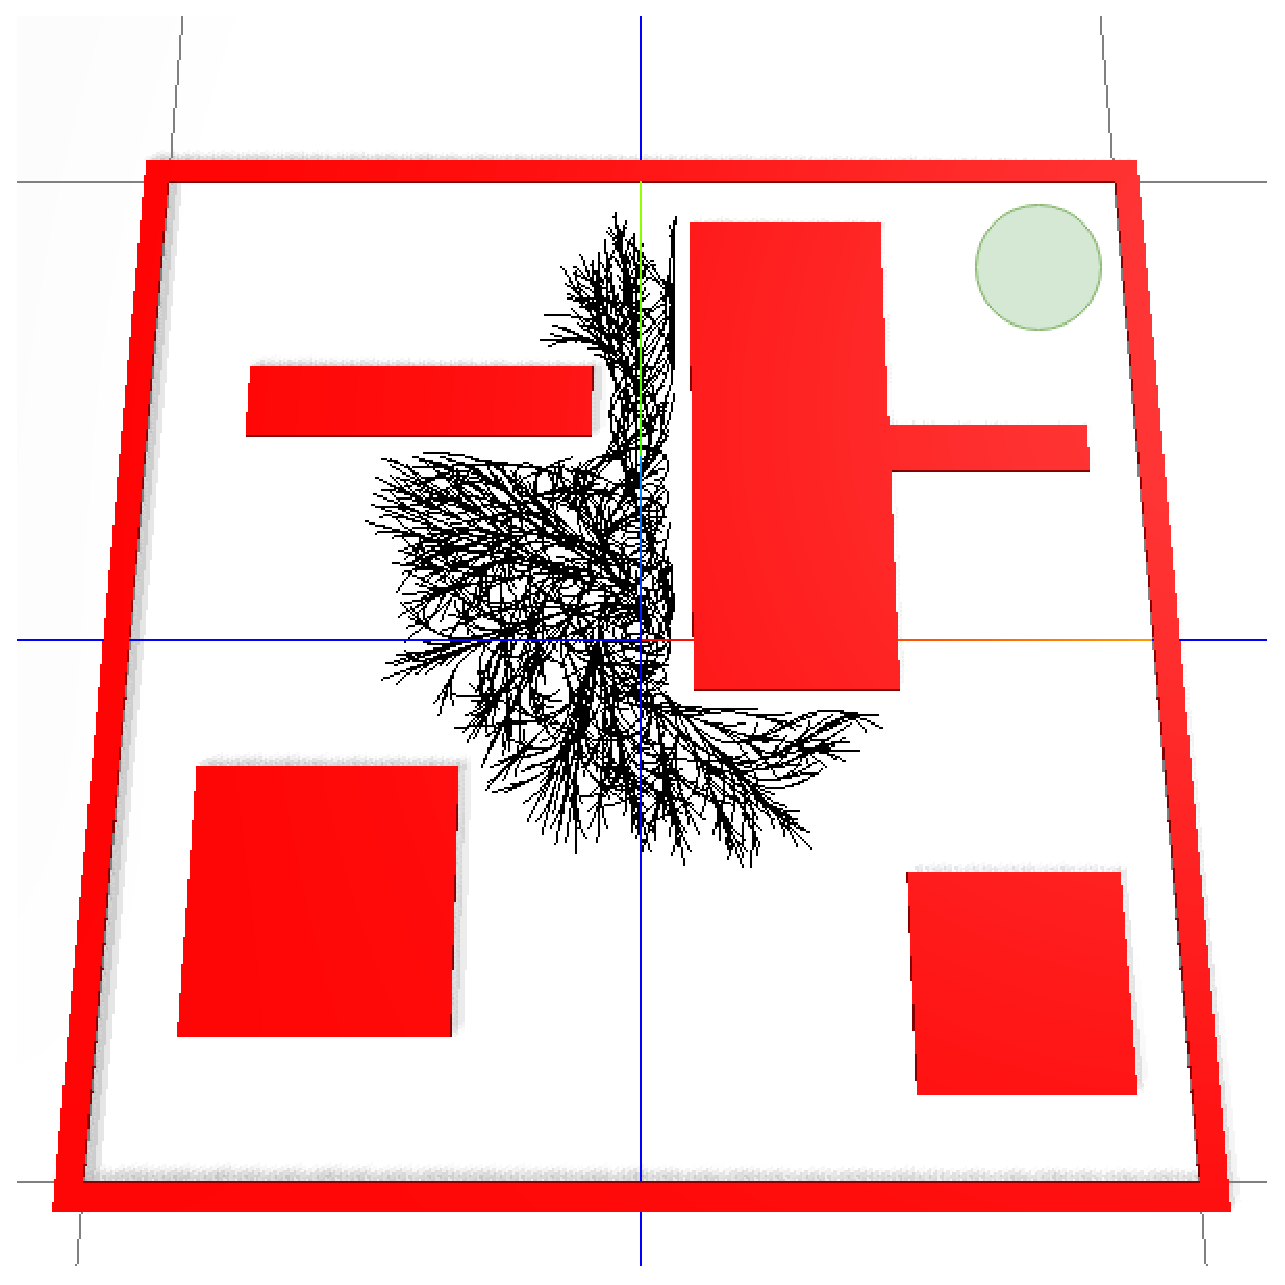
\includegraphics[scale=0.5]{figures/curated.eps}
					\caption{Informed maneuvers navigate the robot (center) to the goal (green) while exploring the workspace. \vspace{-.2in}}
					\end{figure}
			    \end{column}
		    \end{columns}
		\end{block}
	\end{column}
	\begin{column}{0.5\textwidth}
		\begin{block}{\large Motion planning with curated maneuvers}
		    \begin{columns}[T]
		    	\begin{column}{0.38\textwidth}
		    	\begin{figure}
		    	\vspace{-0.2in}
		    	\centering
				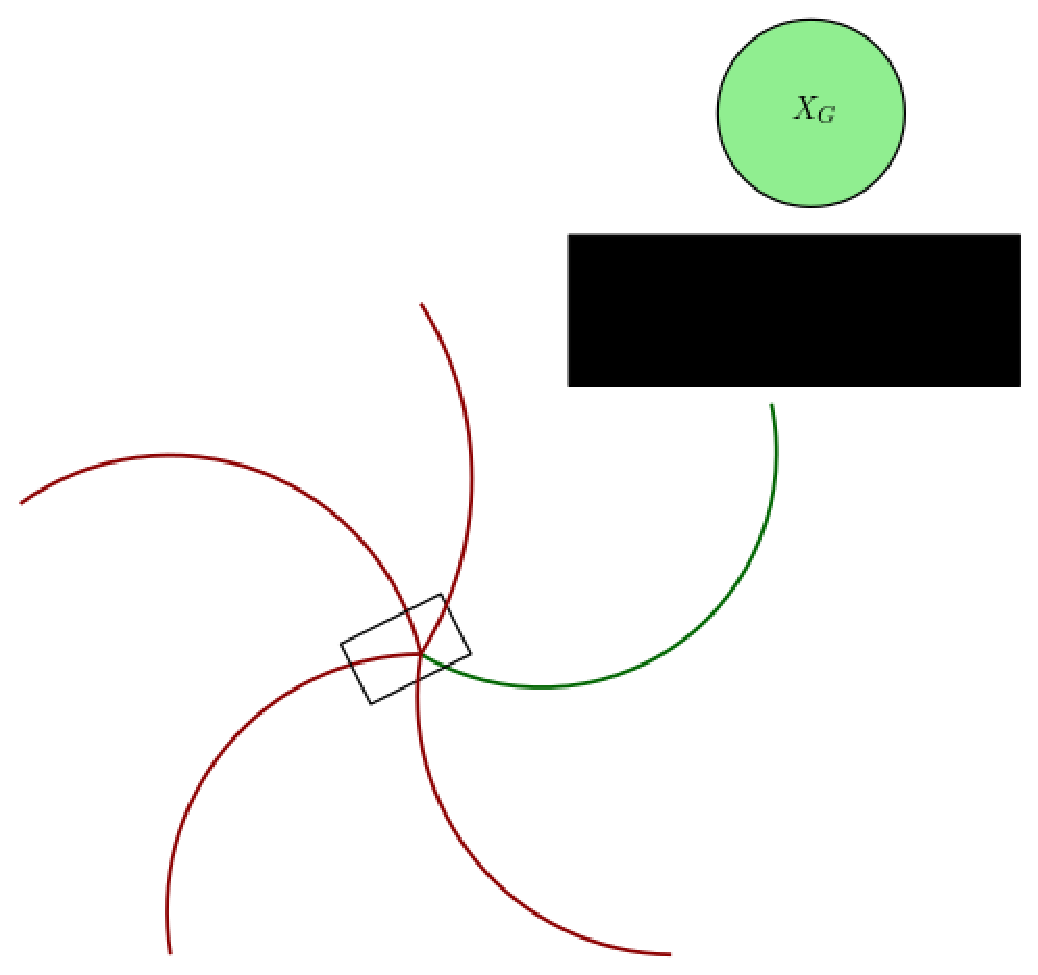
\includegraphics[scale=0.5]{maneuver_sets}
				\caption{From a large set of random maneuvers, the exploitative (green) maneuver minimizes heuristic to the goal (green). Explorative (red) maneuvers are obtained iteratively by maximizing the dispersion to previously curated maneuvers $[2]$. \vspace{-.2in}}
				\end{figure}
		    	\end{column}
		    	\begin{column}{0.6\textwidth}
					% 	\item Informed maneuvers can be computed online employing by using a dispersion metric $[2]$, tailored to each state of the robot selected for propagation. \vspace{0.1in}
		    	\vspace{-0.2in}
					\begin{itemize}
					\item First solution statistics between DIRT using random and curated maneuvers:
					\vspace{0.05in}
					\begin{table}[h!]
						\centering
						\begin{tabular}{|l|l|l|l|}
						\hline
						        & \textbf{Iteration} & \textbf{Time} & \textbf{Path Cost} \\ [0.5ex] \hline
						Random  & 1471                    & 0.2                   & 50.47                  \\ \hline
						Curated & 686                    & 12.15                & 48.13                  \\ \hline
						\end{tabular}
						\vspace{0.05in}
					\end{table}
						\item \textcolor{green}{Very effective in finding a high-quality solution in fewer number of iterations}
						\item \textcolor{red}{Prohibitive to compute online}
						\item \textbf{Goal:} Develop a data-driven approach that achieves the same objective as the curation but can generate the maneuvers fast.
					\end{itemize}
				\end{column}
			\end{columns}
		\end{block}
	\end{column}
\end{columns}	
		    
